\documentclass[11pt,a4paper]{article}
\usepackage[left=2.0cm,top=2.0cm,right=2.0cm,bottom=2.0cm]{geometry} 

\usepackage{graphicx}
\usepackage{amssymb}
\usepackage{epstopdf}
\usepackage{xspace}            
\usepackage{color}
\usepackage{colortbl}
\usepackage{amsmath} % Adds a large collection of math symbols                  
\usepackage{ifthen} % for conditional statements               
\usepackage{amssymb}
\usepackage{amsfonts}
\usepackage{upgreek} % Adds in support for greek letters in roman typeset       
\usepackage{titling}
\usepackage{makecell}
\usepackage{pgfgantt}
\usepackage{lscape}
\usepackage{multirow}
\usepackage{titlesec}
\usepackage{url,amsmath,booktabs,hepunits,abhepexpt,abhep,xcolor}
\usepackage[colorlinks]{hyperref}    % Hyperlinks in references
\usepackage[all]{hypcap} % Internal hyperlinks to floats.
   
\usepackage[bibbreaks=normal, paragraphs=normal, floats=tight, mathspacing=tight, lists=tight, title=tight, margins=normal, wordspacing=normal, tracking=normal, charwidths=normal, bibnotes=normal, mathdisplays=tight, leading=tight, indent=tight, bibliography=normal, sections=tight]{savetrees} 
\renewcommand{\thesection}{\Alph{section}}
\renewcommand{\thesubsection}{\thesection.\arabic{subsection}}

\newboolean{uprightparticles}
\setboolean{uprightparticles}{false} %Set to true to get roman particle symbols

\usepackage{fancyhdr}
\usepackage{rotating}

%\usepackage{fancyheadings}
\pagestyle{fancy}


% Playing with the page size 

\usepackage{array}
\newcolumntype{y}[1]{>{\raggedleft\arraybackslash}p{#1}}

%\renewcommand*{\arraystretch}{1.2}

%TB
%\addtolength{\oddsidemargin}{-10pt}
%\addtolength{\evensidemargin}{-10pt}
%\addtolength{\textwidth}{25pt}
%\addtolength{\textheight}{76pt}
%end TB

%\addtolength{\textfloatsep}{-2pt}
\setlength{\droptitle}{-44mm}

\setlength{\headwidth}{\textwidth}



\newboolean{articletitles}
\setboolean{articletitles}{false}

\usepackage{cite}
\usepackage{mciteplus}

\newboolean{inbibliography}

\titlespacing{\section}{0pt}{4pt}{0pt}
\titlespacing{\subsection}{0pt}{4pt}{0pt}
\titlespacing{\subsubsection}{0pt}{4pt}{0pt}

%\titlespacing{\section}{0pt}{\parskip}{0pt}
%\titlespacing{\subsection}{0pt}{\parskip}{0pt}
%\titlespacing{\subsubsection}{0pt}{\parskip}{0pt}


\title{{\Large Case for ERC starting grant}}
\author{{\normalsize Conor Fitzpatrick}}
\date{}                                           % Activate to display a given date or no date

\usepackage[parfill]{parskip}

\begin{document}

\lhead{{\small Fitzpatrick}}
\chead{{\small Part B2}}
\rhead{{\small Beauty2Charm}}
\begin{center} 

{\Large\bf ERC Starting Grant 2019} \\
 {\Large\bf Research Proposal [Part B2]}  \\
\vspace{2cm} 
\end{center} 

{\Large{\bf Part B2: {\it{The scientific proposal}}}}

\section{State of the art and objectives}
%


\subsection*{Introduction}
The Standard Model (SM) of particle physics is remarkable in that it describes all known fundamental particles and their interactions. It cannot be a complete description of nature however, as it disagrees with cosmological observations as to the nature of matter and energy in the universe. This motivates searches for new particles and evidence of their interactions. The Large Hadron Collider (LHC) is an ideal laboratory for searches of this kind, reaching the highest collision energies of any accelerator to date, it provides a means to create and observe new particles. 

Over the course of the last 8 years, the LHC has made several significant discoveries, including that of a new particle consistent with the SM Higgs Boson. It has yet to find a significant deviation from the Standard Model in searches for beyond the standard model (BSM) physics however, meaning that these new particles must either exist at energies beyond those accessible to the LHC or seldom interact with those of the SM. 

While the on-shell production of new particles at the LHC is limited by the collision energy,  searches for the effects of new particles or fields in quantum processes are sensitive to considerably higher energy scales. One area in particular, namely flavour physics and \CP violation, is of particular interest: \CP violation is required to generate the matter-antimatter asymmetry of the present universe, but the size of the effect observed in the SM is far too small to explain the size of this asymmetry. 
One particularly interesting process to study further is \HepProcess{\PBs-\APBs} mixing, which is mediated by quark flavor changing processes where the small and precisely constrained SM contributions can be enhanced by new physics~\cite{Lenz:2010gu}.

This proposal will look for new physics in \CP observables that are sensitive to new physics in \HepProcess{\PBs-\APBs} mixing, using a family of decays that, until the advent of the \LHCb upgrade and its new trigger, have been impossible to study at the necessary precision. I have played a leading role in both precursors to the proposed measurements and in development of the trigger that will make these measurements possible. 

\subsection{The state-of-the-art}
\subsubsection{The \LHCb experiment at the LHC}
The Large Hadron Collider is the world's largest and highest energy particle accelerator. It collides bunches of protons at center-of-mass energies of up to $14~\TeV$. The LHC schedule is segmented into runs. In Run 1 LHC provided collisions at 7 and $8~\TeV$ between 2010 and early 2013. During Run 2, $13~\TeV$ collisions have been provided from 2015 to 2018. Between these data taking periods, long shutdowns for maintenance and upgrades take place. Long Shutdown 1 (LS1) spanned 2013-2014 during which upgrades were made to the LHC injector chain. LS2 begins at the end of 2018 and will continue until early 2021, at which point the LHC is expected to reach its design energy of $14~\TeV$.

The \LHCb experiment is a single-arm spectrometer fully instrumented in the pseudorapidity range $1.9<\eta<4.9$, designed to exploit the large beauty and charm production cross-sections at the LHC~\cite{Aaij:2014jba}. \LHCb is optimised for studies of decay-time-dependent \CP violation in \PB meson decays, having an excellent vertex and momentum resolution for charged particles together with dedicated particle identification capabilities. One important component of the present \LHCb experiment is its flexible, software higher level trigger (HLT), capable of covering an extremely broad physics programme, from selecting the largest samples of mesons containing charm quarks at high purity to selecting the rarest \PB meson decays containing muons at high efficiency.

During LS2 the \LHCb experiment is undergoing a significant upgrade in order to increase the instantaneous luminosity at which it operates by a factor of five.  This makes the next five years an ideal time to develop improvements to the upgrade, and then collect and analyse data samples of unprecedented sizes.
%and perform analysis with the data these improvements produce.

The \LHCb dataset at the start of this proposal will consist of $8~\invfb$ of \pp collisions collected at the three LHC energies described earlier. Table~\ref{tab:datasets} describes the datasets used in this proposal.
\begin{table}
    \centering
    \begin{tabular}{ccccc}
         LHC Run & years & Collision energy & Size (\invfb) & Run 1 equivalent size (\invfb) \\\hline
         1 & 2010-2012 & 7,8~\TeV & $3$ & $3$\\
         2 & 2015-2018 & 13~\TeV & $5$ & $10$ \\
         3 & 2021-2023 & 14~\TeV & $15$ & $120$ \\
    \end{tabular}
    \caption{Datasets used in this proposal. The Run 1 equivalent size is scaled by the increased cross-section due to higher collision energy, and the effective increase in signal yield due to the trigger efficiency gains delivered by this proposal}
    \label{tab:datasets}
\end{table}

\subsubsection{The \LHCb trigger}
The high $(\sim 30~\MHz)$ \pp collision rate at the LHC and relatively low rate of signals produced per collision mean that all of the LHC experiments make use of a trigger to reject uninteresting collisions and save only those of interest for analysis. At LHCb, in Run1 and Run2 this was achieved using a hardware, low-latency Level-0 trigger which reduces the collision rate to $1~\MHz$ followed by a software HLT running on commodity computing hardware. As project leader of the HLT I am responsible for its current operation and upgrade development. 

\begin{figure}
    \centering
    \includegraphics[width=0.45\textwidth]{figs/L0Eff_Beauty_RUN.pdf}
    \includegraphics[width=0.45\textwidth]{figs/HLT2TotalEff_Beauty_RUN.pdf}
    \caption{LHCb Run 2 Level-0 (left) and HLT (right) efficiencies as a function of run blocks of equal integrated luminosity. The groups separated by spaces correspond to 2015, 2016 and 2017 data taking periods respectively. The Level-0 trigger type is indicated by `Had' for hadronic, `Ele' for electron, `Photon` for photon, and `Mu' and `DiMu' for single- and di-muon triggers respectively.}
    \label{fig:trigger}
\end{figure}
 
The current HLT is extremely efficient for signals triggered by the presence of hadrons in the final state as indicated in Fig.~\ref{fig:trigger}. The Level-0 trigger is not however, as the soft hadrons associated with beauty and charm decays are a challenge to trigger using simple criteria afforded by a fixed-latency hardware trigger. This means that the total trigger efficiency, $\epsilon^{\text{Level-0}}\times\epsilon^{\text{HLT}}$ in Run 2 is as low as 20\% (30\%) for the \HepProcess{\PB\to\PD\PD} (\HepProcess{\PB\to\PD h}) decays relevant to this proposal, motivating a dramatic change in the trigger strategy for the LHCb upgrade.

The PI has developed the groundwork for this change~\cite{LHCb-PUB-2014-027,LHCb-PUB-2014-040,CERN-LHCC-2014-016}, the delivery and full physics exploitation of which is described in this proposal. 
 
\subsubsection{Measurements of beauty production cross-sections}
At the start of a new collider experiment, and at new energies, the rates of production (cross-sections) serve as an important test of QCD hadronisation and fragmentation models. It is vital that these models are understood in order to tune Monte-Carlo generators used in simulation. Due to the unique rapidity coverage of \LHCb measurements of this kind are even more important, as the majority of generator tuning is performed at more central rapidities. \LHCb has made several beauty and charm cross-section measurements at increasing LHC collision energies~\cite{Aaij:2013mga,Aaij:2016jht,Aaij:2015bpa,Aaij:2017qml,Aaij:2013noa}, however to-date these measurements have been limited to either use final states involving muons in the case of beauty hadrons, or, in the case of charm hadrons to short data taking periods at the start of each new running period when the L0 trigger was disabled and replaced with an inefficient random sampling of minimum bias events. The PI has considerable experience of cross-section measurements with final states involving hadrons, having performed one of the first measurements to be presented from \LHCb results at ICHEP in 2010, later published as part of the $7~\TeV$ charm cross-sections~\cite{Aaij:2013mga}.

\subsubsection{Measurements of $\phi_s$ and $\sin(2\beta)$ with \HepProcess{\PB\to\PD\PD} decays}
As indicated in Figure~1 of Part~B1, neutral meson mixing offers unprecedented sensitivity to NP above the energy scales accessible to searches in collider experiments.  A particularly sensitive probe of NP arises in \CPv in the interference between the mixing and decay of \HepProcess{\PBs-\APBs} and \HepProcess{\PBzero-\APBzero} mesons, where the \CP violating weak phase differences $\phi_s=-2\beta_s$ and $2\beta$, where $ \beta = \mathrm{arg}[-V_{cd}V_{cb}^{*}/V_{td}V_{tb}^{*}]$ and $\beta_s =  \mathrm{arg} [-V_{ts}V_{tb}^{*}/V_{cs}V_{cb}^{*}]$ are angles of the \HepProcess{\Pqb-\Pqd} and \HepProcess{\Pqb-\Pqs} unitary triangles. These are constrained to high precision in global fits to the SM~\cite{Koppenburg:2017mad}, any deviation from which would imply the presence of NP entering the mixing diagram. 

The `golden' modes with which these phase differences have been commonly measured to date are \HepProcess{\PBs\to\PJpsi\Pphi} and \HepProcess{\PBzero\to\PJpsi\PKshort}. 
However, these channels are affected by subleading SM contributions, which will become non-negligible at the level of precision anticipated with the \LHCb upgrade~\cite{Liu:2013nea}.
%At the level of precision afforded by \LHCb contributions to the phase difference from additional decay diagrams become non-negligible~\cite{Liu:2013nea}. 
The contribution from these diagrams must be measured as they obscure deviations from the SM prediction by introducing additional phases:

\begin{equation}
\phi_s^{\text{meas.}} = -2\beta_{s} + \phi_s^{\text{NP}} +  \delta\phi_s^{\text{SM}} \, .
\end{equation}

Thus, if the subleading contribution $\delta\phi_s^{\text{SM}}$ is not known sufficiently well, any discrepancy between the measured and predicted values, $\phi_s^{\text{meas.}}$ and $-2\beta_{s}$, cannot be unambiguously interpreted as a new physics contribution $\phi_s^{\text{NP}}$.

\begin{figure}
    \centering
    \includegraphics[width=0.8\textwidth]{figs/penguins.png}
    \caption{Decay topologies contributing to \HepProcess{\PB\to\PD\PD} decays~\cite{Bel:2015wha}}
    \label{fig:penguins}
\end{figure}

The unique feature of \HepProcess{\PB\to\PD\PD} decays is that a full set of channels related by the SU(3) flavour symmetry can be measured, allowing the effects of all the diagrams shown in Fig.~\ref{fig:penguins} to be disentangled.
Thus the value of $\delta\phi^{\text{SM}}_s$ relevant for a determination using the \HepProcess{\PBs\to\PDsplus\PDsminus} channel can be experimentally obtained.
The PI has performed the first measurement of $\phi_s$ in \HepProcess{\PBs\to\PDsplus\PDsminus}~\cite{Aaij:2014ywt}, leading to renewed interest in the theory community~\cite{Jung:2014jfa,Bel:2015wha,Fleischer:2016dqd}.

The state-of-the-art in the \HepProcess{\PB\to\PD\PD} system is shown in Figure~2 of Part~B1, which indicates the size of the SM-allowed region for $-2\beta_{s} + \delta\phi^{\text{SM}}_s$ from~\cite{Jung:2014jfa}, and the \LHCb determination  of $\phi_s^{\text{meas.}}$ using the PI's measurement of \HepProcess{\PBs\to\PDsplus\PDsminus}. 
Since this determination the PI has been responsible as working group convenor for the first measurement of \HepProcess{\PBzero\to\PDplus\PDminus} at \LHCb~\cite{Aaij:2016yip} which resolves the tension between previous BaBar~\cite{Aubert:2008ah} and Belle~\cite{Rohrken:2012ta} measurements. A recent \LHCb paper has also made measurements of $A_\text{CP}$ with \HepProcess{\PBminus\to\PDminus\PDzero} and \HepProcess{\PBminus\to\PDsminus\PDzero} decays~\cite{Aaij:2018dxv}. However, to achieve the future precision indicated in Figure~2 of Part~B1 after this proposal, a complete set of measurements with more data is required. 

\subsubsection{Pinpointing NP with $\gamma$}
The CKM angle $\gamma= \mathrm{arg} [-V_{ud}V_{ub}^{*}/V_{cd}V_{cb}^{*}]$ is unique in that it is the only angle of the CKM unitary triangle that can be determined with decays that proceed exclusively by tree-level amplitudes. 
 Measurements of $\gamma$ in \HepProcess{\PB\to\PD X} decays are experimentally challenging due to the small branching fractions of suppressed decays, with the present world-best measurements having sensitivities no better than $10^{\circ}$. This motivates combining measurements, where the PI has led the world's most precise single-experiment combination using \LHCb data~\cite{Aaij:2016kjh}, recently updated to include another of the PI's publications~\cite{Aaij:2018kpq,Kenzie:2018oob}.
 
 
Two measurements sensitive to $\gamma$ are particularly interesting as they require as input clean measurements of $\phi_s$ and $\sin(2\beta)$. Decay-time-dependent analysis of \CP violation observables in \HepProcess{\PBs\to\PDs\PK} and \HepProcess{\PB\to\PD\Ppi} are sensitive to the combinations $\sin(\phi_s + \gamma)$ and $\sin(2\beta + \gamma)$ respectively. At present sensitivities to $\gamma$~\cite{Aaij:2017lff,Aaij:2018kpq} these are largely unaffected by subleading SM contributions to $\phi_s$ and $\sin(2\beta)$, and so they feature in the global \LHCb $\gamma$ combination. However, with greater sensitivity they provide a means to determine the cause of NP. If deviations from the SM are observed in $\phi_s$ for example, the time-dependent measurement of $\gamma$ in \HepProcess{\PBs\to\PDs\PK} gives an absolutely unique handle to distinguish between NP contributions to \PBs mixing and NP contributions to tree-level \HepProcess{\Pqb\to\Pqc} transitions~\cite{Brod:2014bfa}. Conversely, at future precision, clean measurements of SM $\phi_s$ and $\sin(2\beta)$ will be needed to improve the precision on $\gamma$ from these channels. 

\subsection{Objectives}
As summarised in Part~B1, the proposal is organised into five coherent work packages which logically build using common methodologies to a precision search for new physics with beauty to charm decays. The work packages' main objectives are to: 
\begin{description}
		\item [WP1:] Develop new trigger algorithms beyond the standard paradigm of the \LHCb upgrade. This WP builds on the work that the PI has led as HLT Project Leader in the run up to the data taking in 2021, and it is the first use of a revolutionary implementation of a fully software trigger at a collider experiment.
        \item [WP2:] Perform the first measurements of beauty hadron production cross-sections using decays without leptons. This WP will simultaneously produce measurements that have never been performed and serves as a necessary validation of the trigger system in WP1. In addition, trigger selections to be used in WP5 will be developed. 
        \item [WP3:] Make precise determinations of the SM predictions for the NP-sensitive \CP observables $\phi_s$ and $\sin(2\beta)$ in \HepProcess{\PB\to\PD\PD} decays. This WP includes measurements using both Run~2 and Run~3 data in order to maximise efficient use of time and resources. It will exploit the new trigger paradigm delivered in WP1 and extend the selections delivered in  WP2. 
        \item [WP4:] Make the world's most precise determinations of $\phi_s$ and $\sin(2\beta)$ in \HepProcess{\PBs\to\PDsplus\PDsminus} and \HepProcess{\PBzero\to\PDplus\PDminus} decays, respectively, and through comparison to the determinations of WP3 provide a clean NP search. 
        \item [WP5:] Uncover the structure of the NP measured in WP4 by making the worlds most precise decay-time-dependent determinations of $\gamma$ in \HepProcess{\PBs\to\PDs\PK} and \HepProcess{\PBzero\to\PD\Ppi}. 
        \end{description}
The objectives are described in detail in the following subsections.
\begin{table}
\centering
\begin{tabular}{llll}
        Decay & $BR$ & $\sigma(BR) $ & $\sigma(\CPv)$ \\\hline
        \HepProcess{\PBminus\to\PDminus\PDzero} & $3.8\times10^{-4}$ & $6\%$ & $\sigma(A_{\text{CP}})=1.4\%$\\
        \HepProcess{\PBminus\to\PDsminus\PDzero} & $9.0\times10^{-3}$& $2\%$  & $\sigma(A_{\text{CP}})=0.4\%$\\
        \HepProcess{\APBzero\to\PDsminus\PDplus} & $7.2\times10^{-3}$ & $1\%$  & $\sigma(A_{\text{CP}})=0.4\%$\\
        \HepProcess{\APBs\to\PDminus\PDsplus} & $2.8\times10^{-4}$& $7\%$ & $\sigma(A_{\text{CP}})=4.1\%$\\
        \HepProcess{\PBzero\to\PDminus\PDplus} &$2.1\times10^{-4}$& $5\%$ & $\sigma(\sin2\beta)=3\%$\\
        \HepProcess{\PBs\to\PDsminus\PDsplus} &$4.4\times10^{-3}$& $3\%$ & $\sigma(\sin\phi_s)=3\%$\\
        \HepProcess{\PBzero\to\PDsminus\PDsplus} & $<3.6\times10^{-5}$& $16\%$ & \\
        \HepProcess{\PBs\to\PDminus\PDplus} & $2.2\times10^{-4}$& $7\%$ & \\
        \HepProcess{\PBzero\to\APDzero\PDzero} & $1.4\times10^{-5}$& $15\%$ & \\
        \HepProcess{\PBs\to\APDzero\PDzero} &$1.9\times10^{-4}$& $7\%$ & \\
        \HepProcess{\PBs\to\PDsmp\PKpm} & & & $\sigma(S_{f},S_{\bar{f}})=3\%$ \\
        \HepProcess{\PBzero\to\PDmp\Ppipm} & & & $\sigma(S_{f},S_{\bar{f}})=0.4\%$\\
        \end{tabular}\caption{Extrapolated sensitivities to Branching Ratios (excluding normalisation uncertainties) and \CPv observables described in this proposal. For \HepProcess{\PBzero\to\PDsminus\PDsplus} the current limit is taken as the BR, and for  \HepProcess{\PBminus\to\PDminus\PDzero} the relative BR uncertainty is taken from \HepProcess{\PBminus\to\PDsminus\PDzero}. The combined sensitivity from \HepProcess{\PBs\to\PDs\PK} and \HepProcess{\PBzero\to\PD\Ppi} to $\sin(\gamma)$ corresponds to 6\%. All sensitivities are a factor $\sim2-4$ better than the current best measurements.}
\label{tab:sens}
\end{table}
\subsubsection{WP1: The RTA-enabled upgrade trigger}
The Level-0 trigger is largest source of inefficiency for \HepProcess{\PB\to\PD X} decays of the kind used in this proposal, and is a requirement of the present \LHCb pre-upgrade detector as the readout electronics are limited to a $1~\MHz$ output rate. The upgraded \LHCb experiment removes this readout limitation obviating the need for the Level-0 trigger. The PI has shown that the optimal design of the upgrade trigger is to read out the full LHC collision rate to an all-software trigger similar to the present HLT~\cite{LHCb-PUB-2014-027} enabling real-time analysis (RTA) for the first time at a collider experiment. As project leader of the HLT, the PI is responsible for the development of the trigger for the upgrade~\cite{CERN-LHCC-2014-016}. This in particular makes the proposal timely, as provides the potential for significant gains in sensitivity to \CP observables for \HepProcess{\PBs\to\PDsplus\PDsminus} and \HepProcess{\PBzero\to\PDplus\PDminus} compared to those for \HepProcess{\PBs\to\PJpsi\Pphi} and \HepProcess{\PBzero\to\PJpsi\PKshort} decays.

\begin{figure}
    \centering
    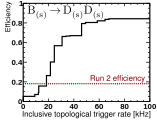
\includegraphics[width=0.7\textwidth]{figs/dsds_topo-crop.pdf}
    \caption{Run 2 inclusive topological trigger efficiency as a function of output rate using Run 3 simulated signal~\cite{LHCb-PUB-2014-040}. The Run 2 Level-0$\times$HLT efficiency for \HepProcess{\PB\to\PD\PD} decays is shown, along with the acceptable output rate for the Run 3 topological trigger. The performance improvements enabled by this proposal lead to the efficiency indicated in green.}
    \label{fig:topo}
\end{figure}

In the RTA paradigm, the detector is fully aligned and calibrated prior to reconstruction, and trigger selections are only then applied to the fully reconstructed, calibrated and aligned collisions. This is conceptually different to the normal trigger paradigm at a collider experiment, where trigger selections are applied prior to complete reconstruction, using a subset of the information. 

In WP1 the PI will develop the RTA methodologies needed to make full use of the increased signal efficiency afforded by removal of the Level-0 trigger. In particular, the increase in luminosity means that the current Run 2 HLT is insufficient to recover the full efficiency: The present HLT selects \PB meson decays using an inclusive topological trigger which looks for 2, 3, and 4 track combinations consistent with a partially reconstructed \Pqb hadron  decay~\cite{Gligorov:1384380}. In Run 2 this is highly efficient for \PB mesons that have been selected by Level-0, but in Run 3 the increased signal rate saturates the available output bandwidth from the trigger, resulting in only a marginal increase in efficiency with respect to Run 2 as shown in Figure~\ref{fig:topo}. 

WP1 will develop the framework with which the first truly RTA enabled trigger selections can be written. Exclusive selections will be developed for the entire range of \HepProcess{\PB\to\PD X} decays required for the remainder of the proposal in WP2. 
With these RTA-enabled trigger selections, further reconstruction is no longer needed 'offline', prior to analysis. The information saved from the trigger can be reduced to only the part of the event that is used in the analysis itself, meaning the raw detector hits, additional tracks and primary vertices can be removed from the event. This leads to a significant reduction in the event size that has to be sent to disk from the trigger. {\bf{As the output limitation is one of bandwidth, not of rate, a reduction in the event size permits a commensurate increase in event rate, recovering the full efficiency gain made available by removal of the Level-0 trigger.}}

A significant challenge in WP1 is to ensure that the data that is saved in the RTA paradigm is sufficient for analysis. In particular for decay-time-dependent analyses of neutral \PB meson decays, knowledge of whether the initial state corresponds to $\PB^{0}_{(s)}$ or  $\APB{}^{0}_{(s)}$ must be inferred by flavor tagging~\cite{Aaij:2012mu}. This requires that the flavor tagging algorithms, normally applied offline after the data have been recorded, must be applied as part of a real-time trigger, and sufficient information must be stored for later calibration.


Successful delivery of this paradigm will result in \LHCb being the only experiment capable of collecting large samples of the flavor tagged $\PB^{0}_{(s)}$ meson decays needed for this proposal, and will also make it the only LHC experiment in Run 3 able to efficiently trigger and record the entire range of \HepProcess{\PB\to\PD X} decays. \textbf{The reduction in bandwidth afforded by RTA development in WP1 will permit up to a factor of four increase in selection efficiencies for WP2-WP5 with respect to the Run 2 trigger.}

\subsubsection{WP2: Cross-section measurements enabled by RTA}
A major advantage of the RTA paradigm is its increased flexibility. Removal of the Level-0 trigger removes the largest source of systematic uncertainty for absolute cross-section measurements as Monte-Carlo simulation, used for absolute efficiency determinations, has previously struggled to model the behavior of the Level-0 hadron trigger. This allows, for the first time ever, cross-section measurements to be made at a hadron collider using final states that do not contain leptons. 
Measurements of production cross-sections with hadronic final states will test every aspect of our detector reconstruction, alignment, and calibration, and are therefore crucial for enabling the physics objectives of the subsequent work packages.

The objective of WP2 is to determine the inclusive production cross-sections in $14~\TeV$ \pp collisions of \Pqb hadrons using four \HepProcess{\PB\to\PD X} decay modes:
\HepProcess{\PBminus\to\PDzero\Ppiminus}, 
\HepProcess{\APBzero\to\PDplus\Ppiminus}, \HepProcess{\APBs\to\PDsplus\Ppiminus} and \HepProcess{\PbgL\to\PLambdac\Ppiminus}. 
The results will be of broad interest to the \LHCb physics programme, and will be of high impact as they will be critical for the tuning of Monte-Carlo generators.
WP2 is also important to define and commission the selections to be used by the remainder of the project, the decay modes for which are indicated in Table~\ref{tab:sens}.

\textbf{The cross-section measurements in WP2 will be the first \Pqb-hadron cross-section measurements at $14~\TeV$, and the first without leptons in the final state.}

\subsubsection{WP3: Determining SM contributions to \CP observables in \HepProcess{\PB\to\PD\PD}}

In order to find new physics in the \HepProcess{\PB\to\PD\PD} system, the size of the SM contributions to mixing-sensitive observables from decay amplitudes shown in Fig~\ref{fig:penguins} must be measured. This is the objective of  WP3, which will follow the strategy set out in Ref.~\cite{Jung:2014jfa}. 

By measuring Branching Ratios (BRs) and direct \CP asymmetries ($A_{\text{CP}}$), SU(3) flavour symmetry relations can be used to determine the expected contributions to measurements of $\phi_s$ and $\sin2\beta$. Additional quasi-isospin relations can be used to test consistency between the measurements and yield predictions. 

WP3 will result in precise measurements of ten BR and four $A_{\text{CP}}$ values, as shown in Table~\ref{tab:sens}, using the Run 2 and first year of Run 3 datasets where the sensitivities shown are extrapolated from existing measurements and Table~\ref{tab:datasets}.  Each of the BR and $A_{\text{CP}}$ measurements will be the world's most precise. Notably, as part of WP3 a first observation of the suppressed decay \HepProcess{\PBzero\to\PDsplus\PDsminus}, which is of particular interest to evaluate the impact of the suppressed `E' and `PA' diagrams of Fig.~\ref{fig:penguins}, is anticipated.
%and the first time-dependent measurement of $A_\text{\CP}$ in \HepProcess{\APBs\to\PDminus\PDsplus} will be made.

\textbf{The objective of WP3 is to reduce the uncertainty on the SM contribution to NP-sensitive observables far below the statistical sensitivity that measurements of these observables will reach, allowing direct comparison between the SM and measurements in WP4.} The size of potential SM contributions to $\phi_s$ before and after WP3 is indicated in Figure~2 of Part~B1.

\subsubsection{WP4: Time-dependent analyses of \HepProcess{\PBzero\to\PDplus\PDminus} and \HepProcess{\PBs\to\PDsplus\PDsminus} decays}
Work within WP4 will result in the world's best measurements of NP-sensitive observables $\phi_s$ and $\sin2\beta$ in \HepProcess{\PBs\to\PDsplus\PDsminus} and \HepProcess{\PBzero\to\PDplus\PDminus} decays, respectively, through decay-time-dependent analyses using the full Run 3 dataset.

\textbf{The objective of WP4 is to measure the NP-sensitive observables $\phi_s$ and $\sin2\beta$ to 3\% precision and compare them to the predictions of WP3}. Deviations between the measurements made in WP4 and the predictions made in WP3 would be an unambiguous signal of new physics.

\subsubsection{WP5: Time-dependent analyses of \HepProcess{\PBs\to\PDs\PK} and \HepProcess{\PBzero\to\PD\Ppi} decays}

WP5 serves two different objectives depending on the outcome of WP3 and WP4: If deviations from the SM are observed in the interplay between the determinations of the observables in these two WPs, confirmation of this deviation is provided and the type of NP process is uncovered through tests of deviations in measurements of $\sin(\phis+\gamma)$ and $\sin(2\beta+\gamma)$. If $\gamma$ is found to be consistent with the SM expectation when using $\phi_s$ and $\sin2\beta$ determined from WP4, and inconsistent with WP3, this will imply new physics in mixing. Conversely if the results of WP3 and WP4 are consistent with the SM, the measurements of WP5 will be used to enhance the precision to which $\gamma$ is known. 

\textbf{The objective of WP5 is to make precise determinations of $\sin(\phis+\gamma)$ and $\sin(2\beta+\gamma)$ to uncover the cause of NP observed with WP4.}

\section{Methodology}

\subsection{Common Methodologies}
The work carried out in WP1-5 builds logically, meaning that tools and techniques developed to make measurements in earlier work packages are also used and further developed in later ones. This proven methodology builds on the PI's extensive track record of world-best measurements. I describe here the methodology common to several work packages:


\subsubsection{Signal selection}
\label{sec:sels}
Selections consist of applying criteria to the data that preferentially retain signal while rejecting background. The trigger is a form of selection, for example. The Run 2 data, which will be used for analysis in advance of Run 3 data taking, has already been selected by the topological trigger, resulting in a pure sample of \Pqb-hadrons. It must be further selected to retain only the decays of interest to this proposal. Exclusive selections designed to reduce the inclusive trigger output to only the decays of interest will be developed, which will form the foundational basis for the upgrade trigger selections which will be deployed as part of WP2 and WP3.  

In WP2 the full set of selections for the \HepProcess{\PB\to\PD X} decays used in WP2 and WP5 will be developed as these can be defined using common components and applied in parallel.
Selections for WP2 begin with combinations of charmed mesons using common selection criteria. The \HepProcess{\PDpm} and \HepProcess{\PDspm} candidates will be reconstructed in \HepProcess{\PK\PK\Ppi}, \HepProcess{\PK\Ppi\Ppi} and \HepProcess{\Ppi\Ppi\Ppi} final states. Using multiple charm final states  both increases the statistical precision of the analyses and provides an internal cross-check of the particle ID performance. Similarly for \HepProcess{\PDzero} modes 2- and 4- body final states will be reconstructed, which provides an additional cross-check of the tracking efficiency performance. From these common final states, the specific \Pqb~hadron can be constructed with the addition of a kaon or pion.
WP3 will then develop the remaining selections making combinations of the common charm final states. 
The selections developed in WP3 in combination with experience gained from WP2 will directly and efficiently translate into RTA trigger selections ready for data taking for the remainder of the project.

\subsubsection{Analysis framework and fitting}
\label{sec:fits}
From WP2 onwards, signal yields and \CP observables will need to be inferred from the data. These will be determined via likelihood fits to probability density functions (PDFs) modelling the signal and background components. These fits will be built within a common analysis framework that will be extended from WP2-WP5, with the majority of the analysis framework being developed in WP3. 

Signal yield determinations will be made using fits to the invariant mass of the \HepProcess{\PD\PD} or \HepProcess{\PD h} decay distributions. The PDF shapes will be modelled using Monte Carlo, where experience has shown that differences between MC and data can be accounted for directly in the fit procedure.

Time-integrated \CP asymmetries in WP3 will be measured by extending the fit to perform simultaneous likelihood fits to, for example, the \HepProcess{\PDzero\PDminus} and \HepProcess{\APDzero\PDplus} invariant mass distributions using common signal and background shapes to extract yield asymmetries. WP3 will further extend the fitting framework to incorporate decay time dependence for determinations of time-dependent \CP asymmetries. 

Care will be taken to ensure that the analysis framework is adaptable, maintainable, reproducible and documented, as the framework will be relied upon for the full project timescale. 

\subsubsection{Common signal and control channels}
\label{sec:controls}
Analysis of the decay modes in a unified manner removes the distinction between signal and control modes. For example, the decay \HepProcess{\APBzero\to\PDsminus\PDplus} serves as a control channel from which the decay time acceptance is determined for \HepProcess{\PBs\to\PDsplus\PDsminus} and \HepProcess{\PBzero\to\PDplus\PDminus} decays, while it will be used in advance as part of the branching ratio and direct \CP asymmetry measurements. By developing the selections, signal modelling and fitting components for all of the modes together consistency in treatment is guaranteed. 

\subsubsection{Pseudoexperiments and Monte-Carlo simulation}
\label{sec:MC}
In order to develop the fitting framework, study selections and determine systematic uncertainties, simulated samples of signal and background decays that have been propagated through a model of the \LHCb detector, trigger and reconstruction are required. At \LHCb these simulated samples are produced centrally using grid computing resources. Monte-Carlo simulation requests must be made well in advance and tested to ensure that they are available in a timely fashion. 
The Warwick group contains significant expertise on the \LHCb simulation, which can be exploited to avoid unnecessary delays due to simulation production.

In WP2 the full set of \HepProcess{\PB\to\PD X} modes needed for both WP2 and WP5 will be requested under Run 3 conditions as several WP2 decay channels are control channels for WP5. 
In WP3 the set of simulated Run 2 and Run 3 samples necessary for the remainder of the project will be produced, as simulated samples used for the BR measurements are the same as those used for the decay-time-dependent and decay-time-integrated analyses of WP3 and 4.

Pseudoexperiments, also referred to as `toys' in the literature, consist of fast simulation derived from distributions. These will be used extensively throughout the course of the proposal to validate the fit and derive systematic uncertainties associated with imperfect modelling of signal components. The ability to generate pseudoexperiments will be developed in the analysis framework in WP2, and will be used in WP2-5. Due to the high signal yields afforded by the \LHCb upgrade and enabled by the RTA trigger in this proposal, pseudoexperiment studies will be computationally intensive and will make use of the Elementary Particle Physics group computing cluster at Warwick for which additional funds and a contribution towards administration are requested.

\subsection{Project planning}
\begin{figure}[h!]
\begin{center}
\includegraphics[width=\textwidth]{figs/Gantt_B2_forPublication.pdf}
\caption{\label{fig:timeline} Detailed project timeline describing the allocation of team members and work package durations. Vertical lines indicate dependencies between work packages. Publications are marked with yellow diamonds.}
\end{center}
\end{figure}

The research team will be comprised of the PI, a PDRA, and three PhD students. In the following, a detailed description of the work to be undertaken by the team is given. 

A timeline describing the overall planning and allocation of team members is provided in Figure~\ref{fig:timeline}. This has been prepared using project planning and management software~\cite{omni:plan}, taking particular care to schedule tasks common to all analyses and balancing the work between the research team in a way that ensures the ambitious project is achievable within the timescale and resources of this research proposal. Resources are discussed in the next section.

\subsubsection{WP1: Upgrade trigger development}
In WP1 the PI will work with PhD1 to enable the full output of the topological trigger to be used input to a final trigger stage that selects the exclusive signal decays. Once selected, only the tracks, vertices, mass hypotheses and particle ID information are needed at the analysis stage for branching fraction measurements. For neutral \PB meson decay modes a challenge will be in saving  additional information required to tag the initial flavor. The PDRA will develop real-time flavor tagging for use in the trigger, and determine which additional components of the event should be stored offline for flavor tagging calibration. PhD1 will be based at CERN from Q3 2020 to Q3 2021 in order to work with the commissioning team to install the flavor tagging and selection framework for the RTA trigger, and to participate in the first data taking. 

At the start of 2021, the selection and real-time flavor-tagging framework will be delivered, ready for  the commissioning period with beam where the PI, PDRA and PhD1 will monitor the selection operation and  performance prior to stable data taking. 

Three deliverables are foreseen in WP1: A commissioning paper which will describe the new RTA paradigm in detail, to be published shortly after the start of data taking in Q2 2021,
%marked with <1>
a trigger performance paper to be published in Q4 2021 
%marked with <2>
highlighting the selection and reconstruction efficiencies of the RTA trigger similar to~\cite{Aaij:2012me}, and a chapter in a more general \LHCb upgrade paper in Q2 2022 similar to~\cite{Aaij:2014jba} which will summarise the performance. 
%marked with <3>

Given the importance of the trigger commissioning and its reliable operation not just for this proposal but for the entire \LHCb physics programme, the PhD students in this project will be trained as RTA experts by the PI and PDRA. They will spend time during their secondments at CERN contributing to the ongoing development and operation of the trigger during data taking.  

\subsubsection{WP2: Commissioning the RTA paradigm}

By developing the cross-section analysis prior to commissioning, throughout Q1-Q3 2020, the analysis framework can be made ready to run from the start of data taking as the first true application of RTA. As an RTA analysis, it is robust against schedule changes or lower than expected luminosities from the LHC: Once the necessary trigger selections have been commissioned by the PI, PhD1 and PDRA, they can run transparently with the rest of the \LHCb physics programme until a sufficient sample size has been collected, at which point the pre-written analysis framework can be run without delay, reducing time to insight.

PhD1 will work with the PI to develop a fully reproducible analysis, making the first version of the  analysis framework described in section~\ref{sec:fits}. Monte-Carlo samples will be requested as described section~\ref{sec:MC}. In combination with the preexisting Run 2 data this will be used to define the first selections (sec.~\ref{sec:sels}) and will be used to develop invariant mass fits from which background subtraction can be performed in order to determine the raw signal yields in bins of $\pT$ and $\eta$. When applied to the data at the start of Run 3, Monte Carlo will be used to obtain efficiency corrected yields from which the doubly-differential cross-sections can be calculated automatically.

Once the framework has been fully tested, the selections determined from the Monte Carlo and Run~2 datasets will be installed in the trigger framework developed in WP1. This will happen well in advance of data taking which starts in Q2 2021.

The WP2 preparation will proceed in parallel with trigger developments, and be ready for data sufficiently early that the PI and PhD1 will be free to focus on commissioning at the critical time from Q3 2020 to Q2 2021 when global readiness tests of the upgrade detector and trigger will require the full attention of the project members. PhD1 will be present at CERN during the data taking, and will monitor the progress of the early measurements as data is collected. 

The deliverable for this work package is the publication of beauty-hadron cross-sections at $14~\TeV$ using the first data with the upgraded \LHCb detector in Q4 2021 ready for the winter conferences in Q1 2022. 
%marked with <4>
In order to ensure rapid dissemination of the results and ease-of-use for generator tuning, the cross-sections will be made available via HepData~\cite{Maguire:2017ypu} and as Rivet~\cite{Buckley:2010ar} plugins. The limiting systematic uncertainty is likely to be the precision to which the luminosity can be measured in the early data. This is expected to be better than a few $\%$. 

\subsubsection{WP3: Determining SM contributions to \CP observables in \HepProcess{\PB\to\PD\PD}}
WP3 begins at a time when the research team is at its full compliment, with PhD1 and PhD2 both active. In this Work Package the fitting framework is finalised for the remainder of the project. It is divided into 3 deliverables, which will be carried out by PhD1, PhD2, the PI and the PDRA:

\paragraph{Determination of Branching Ratios:}
\label{sec:BRs}
The first deliverable of WP3 will be carried out by PhD2 and the PI. It begins with a literature review by PhD2, leading to development of the Monte-Carlo simulation requests for WP3 onwards described in section~\ref{sec:MC}, and continues with optimisation of the common selections described in section.~\ref{sec:sels}. At this stage care must be taken to ensure that the selections are not only efficient and pure, but that they are suitable for the time-dependent analyses in later work packages. PhD2 will, with training from the PI, will pay careful attention to decay time acceptance distributions. The selections will be ready to be installed in the trigger by Q1 2021. 

The branching ratio analysis will be performed on the pre-existing Run 2 dataset, and will further develop the analysis framework that has been deployed in WP2. Signal yields will be determined from likelihood fits to the invariant mass distributions for the ten decay modes listed, with shapes determined from Monte Carlo and informed by previous measurements. In the case of \HepProcess{\PBzero\to\PDsplus\PDsminus} a limit will be set in the case that the signal is insufficient to claim first evidence, and a second publication will be considered later in the project by PhD3 using the Run 3 data if necessary. Branching fractions will be determined based on the signal yields, with \HepProcess{\PBminus\to\PDsminus\PDzero} as a normalisation channel, benefitting from the common signal and control channel strategy described in section~\ref{sec:controls}. This will lead to a publication covering the ten BRs in Q1 2022. 
%marked with <5>

\paragraph{$A_{\text{CP}}$ measurements with \HepProcess{\PBminus\to\PDminus\PDzero} and \HepProcess{\PBminus\to\PDsminus\PDzero}:}
By Q4 2021 PhD1 will have returned from CERN to Warwick, where they will begin work on $A_{\text{CP}}$ measurements in the  \HepProcess{\PBminus\to\PDminus\PDzero} and \HepProcess{\PBminus\to\PDsminus\PDzero} channels, with supervision from the PI. These are functionally identical and so proceed in parallel as a single analysis. Using the invariant mass fit models developed for the branching ratio measurements, the student will update the fitting framework to perform simultaneous fits of the same models split by $\PBpm$ charge. As an expert in data taking operations for Run 3, they will process the first year of data recorded with the upgraded detector, and include this in the fit, also making it available to PhD2 for the \PBzero $A_{\text{CP}}$ measurements.
A significant challenge in this analysis will be determination of detection and production asymmetries and control of the corresponding systematic uncertainties, which will require pseudoexperiments as described in section~\ref{sec:MC}. The Run 3 data will benefit from the RTA paradigm as it will have a reduced detection asymmetry systematic uncertainty. A significant fraction of the uncertainty in previous measurements has been due to the Level-0 trigger which will no longer be present.  A publication of $A_{\text{CP}}$ measurements with the charged modes will be made in Q2 2022, 
%marked with <6>
at which point PhD1 will write their thesis. 

\paragraph{$A_{\text{CP}}$ measurements with \HepProcess{\APBs\to\PDminus\PDsplus} and \HepProcess{\APBzero\to\PDsminus\PDplus}:}
In parallel PhD2 will begin work on $A_\text{CP}$ measurements with the neutral \PB modes \HepProcess{\APBs\to\PDminus\PDsplus} and \HepProcess{\APBzero\to\PDsminus\PDplus}. As \HepProcess{\APBzero\to\PDsminus\PDplus} is an important control channel for the time-dependent measurements,  PhD2 will further extend the common fitting framework to include the decay time dependency from which time-dependent \CP observables can be extracted in later work packages.
Although these decay modes are flavor specific, and hence decay-time-dependent analysis is not necessary to determine $A_\text{CP}$, this procedure will be invaluable to verify the fit procedure and will also improve the sensitivity through better separation of the signals from background. This will involve inclusion of the flavour tagging and so proceeds under the supervision of the PDRA, whose expertise in developing the real-time flavour tagging developments for the Run 3 trigger will be invaluable. PhD2 will be based at CERN from Q3 2021 - Q3 2023 in order to be trained in RTA data taking operations and to embed in the \LHCb Beauty to Open Charm (Time-Dependent) working group where time-dependent analyses of this kind are developed, and in the Flavor tagging performance working group where they will be responsible for delivering the flavor tagging performance studies needed for this proposal  and other analyses ongoing in the \LHCb collaboration. The expertise in the working group at CERN will accelerate the development of the fitting framework and allow the student to contribute to the Run 3 data taking and performance activities.

The PDRA and PhD2 will work together to determine and automate the evaluation of additional systematic uncertainties associated with time-dependent analyses. It is critical that these are developed in a reproducible manner as the techniques developed will be used additionally in WP4 and WP5. In addition to the systematic uncertainties associated with the flavour tagging calibration, measurements of the decay time resolution and decay time acceptance are required. These will be added to the analysis framework for continued use.

Publication of the $A_{\text{CP}}$ measurements of \HepProcess{\APBs\to\PDminus\PDsplus} and \HepProcess{\APBzero\to\PDsminus\PDplus} will occur in Q3 2022.
%marked as <7>

\subsubsection{WP4: Searching for NP in decay-time-dependent analyses}

In Q4 2022, the PI will arrange for theorists who have published papers relevant to this proposal to attend the \LHCb-hosted implications workshop at CERN to discuss the outcomes of WP3 with a view to developing updated predictions of the NP-allowed sensitivities for \HepProcess{\PB\to\PD\PD} decays with the first year of Run 3 data. Quasi-isospin relations will be used to test agreement between the WP3 measurements and develop predictions for the SM expectation for the direct measurements to be carried out in WP4.

Measurements of $\phi_s$ and $\sin(2\beta)$ will begin in Q3 2022 with the Run3 data accumulated during 2021 and 2022. The fitting and systematic uncertainty determinations will have been informed by the developments in WP3, and will proceed using the now complete fitting framework. The PI with PhD2 and the PDRA with PhD3 will perform these first measurements of $\sin2\beta$ and $\phi_s$ leading to two simultaneous publications in Q1 2023 ready for winter conferences.
%marked as <8>

The final year of data taking in Run 3 is expected to double the size of the Run 3 dataset which will be incorporated leading to two publications in Q1 2024 led by the PDRA and PhD3 under joint supervision of the PI. At this point, the precision on $\phi_s$ and $\sin2\beta$ will be that listed in Table~\ref{tab:sens}. The PI will have started work on a review paper to be ready for Q3 2024 in which the updated predictions determined from WP3 results will be compared to quantitatively with those of WP4. 
%marked as <9>

\subsubsection{WP5: Null-tests of the SM with clean measurements of $\gamma$}

 In WP5, the PI, PDRA and PhD3 will perform measurements of $\sin(2\beta + \gamma)$ and $\sin(\phi_s + \gamma)$ in \HepProcess{\PBzero\to\PD\Ppi}  and \HepProcess{\PBs\to\PDs\PK} respectively. These measurements will use the same time-dependent fitting framework developed in WP3 and selections derived from and commissioned in WP2, meaning that they can proceed in a timely fashion. The measurement using \HepProcess{\PBzero\to\PD\Ppi} is slightly more straightforward as flavor tagging calibrations for this mode can be determined directly from the fit to the data. The results of these fits can be used in two ways: In combination with additional results from \LHCb, the world's most precise single-experiment measurement of $\gamma$ will be available, with an expected precision of $1^{\circ}$. By including the WP4 measurements of $\phi_s$ and $\sin 2\beta$ the extracted values of $\gamma$ can be checked for tension with the tree-level only determinations of $\gamma$ which are entirely free of theoretical uncertainty. Tension would enhance the case for the presence of new physics in \HepProcess{\PB\to\PD\PD} decays. In the absence of any tension, the combination of WP4 and WP5 would improve the SM determination of $\gamma$, and would ensure that the size of SM pollution contributing to the world average is fully controlled.
 
 Much of the WP5 preparation, including preliminary blinded fits to the 2021 and 2022 datasets can proceed in parallel with WP4, with PhD3 starting work after the fitting development is complete in WP3 in Q4 2021. The main body of work in determining systematic uncertainties and incorporating the last year of Run 3 data will begin in Q2 2023, with two publications at the end of the proposal in Q3 2024. 
 The measurements made in WP5 will be incorporated into the review paper to be published by the PI at the end of Q3 2024, marking the successful completion of the proposal.   
%marked as <10>

\subsection{Risks} 

\subsubsection{Delays to the LHC and LHCb data taking schedule}
WP1 and the Branching Ratio measurements described in WP3 do not rely on Run 3 data. These are unaffected by delays to the LHC and LHCb data taking schedule. In case of a delay, hiring of PhD2 may be deferred by up to six months, at which point only a six month delay to publications of the $A_{\text{CP}}$ measurements would result, with PhD1 developing the fitting framework in WP3 in place of PhD2 and in advance of the inclusion of Run 3 data. WP2 preparations must be ready in time for nominal data taking, at which point publication can be deferred until sufficient data is collected without impact to the other work packages. 
\subsubsection{Reduced RTA functionality}
The Run 3 trigger must process the full $30~\MHz$ of collisions in real-time in software using commodity computing nodes. This is expected to be challenging with the available \LHCb upgrade computing budget. The PI, PDRA and PhD1 will expend significant effort in the trigger development and commissioning stages to ensure that a sustained $30~\MHz$ throughput is achieved from the start of data taking. The first year of Run 3 is expected to be a commissioning year, in which \LHCb may run at a lower luminosity than in 2022 and 2023. The extrapolations in Table~\ref{tab:sens} account for this, and the reduced luminosity would mitigate any performance shortfall in the first year which will be made up in the second when \LHCb purchases additional servers. However, in the case of a continued shortfall, I have developed strategies to mitigate up to a 50\% reduction in computing performance while retaining 90\% efficiency for the signals of interest to this proposal~\cite{Bourgeois:2018nvk}. This mitigation can be deployed during the commissioning period as part of WP1.


\section{Resources}
\begin{table}[!htb]
\setlength{\extrarowheight}{2pt}
  \centering
  \caption{Summary of the requested resources.}
  \label{tab:resources}
  \begin{tabular}{|l|l|l|r|}\hline
    \multicolumn{3}{|l|}{\bfseries Cost Category} & {\bfseries Total (in euros)} \\ \hline
    \multirow{12}{*}{\bfseries Direct Costs} & \multirow{5}{*}{\bfseries Personnel} & PI (see text) & 329\,263  \\ \cline{3-4}
                                       &                                & Senior Staff & 0 \\ \cline{3-4}
                                       &                                & Postdocs     &  333\,457 \\ \cline{3-4}
                                       &                                & Students     &  156\,780 \\ \cline{3-4}
                                       &                                & Other        &  81\,166  \\ \cline{2-4}
                                       & \multicolumn{2}{|l|}{\itshape i. Total Direct Costs for Personnel (in euros)} & 900\,666 \\\cline{2-4}
                                       & \multicolumn{2}{|l|}{\bfseries Travel} &  169\,650 \\\cline{2-4}
                                       & \multicolumn{2}{|l|}{\bfseries Equipment} &  65\,000  \\\cline{2-4}
                                       & \multirow{3}{*}{\bfseries Other goods and services} & Audit              &  5\,850 \\\cline{3-4}
                                       &                                & Recruitment        &   2\,600   \\\cline{3-4}
                                       &                                & Training        &   39\,000   \\\cline{3-4}
                                       &                                & Consumables        &   16\,250   \\\cline{3-4}
                                       & \multicolumn{2}{|l|}{\itshape ii. Total Other Direct Costs (in Euro)} & 298\,350 \\ \hline
    \multicolumn{3}{|l|}{{\bfseries A - Total Direct Costs (i+ii)}}  & 1\,199\,016 \\ \hline
    \multicolumn{3}{|l|}{{\bfseries B - Indirect Costs (overheads)} 25\% of Direct Costs }  & 299\,754 \\ \hline
    \multicolumn{3}{|l|}{{\bfseries C1 - Subcontracting Costs} (no overheads)}  & 0  \\ \hline
    \multicolumn{3}{|l|}{{\bfseries C2 - Other Direct Costs} (no overheads)}  & 0 \\ \hline
    \multicolumn{3}{|l|}{{\bfseries Total Estimated Eligible Costs (A+B+C)}}  & 1\,498\,770 \\ \hline
    \multicolumn{3}{|l|}{{\bfseries Total Requested EU Contribution }}  &   1\,498\,770  \\ \hline
  \end{tabular}

\vspace{0.3cm}
  \begin{tabular}{|l|c|}\hline
     \bfseries Duration of the project in months & 60 \\ \hline
     \bfseries Time of the PI dedicated to the project over grant period & 100\% \\ \hline
  \end{tabular}
\end{table}

The resources requested for this proposal are listed in Table~\ref{tab:resources} and described in detail below. 

\subsection{Personnel}

\subsubsection{Principal Investigator} 
As PI I will coordinate the project, and supervise the work of the PDRA and PhD students. I will continue to develop the shared analysis software used to extract time-dependent \CPv observables and to develop the machine learning software needed for optimisation of trigger resources. At the start of the proposal I will develop the cross-section measurements as these will be time critical in order to be ready for the first data. As PI, I will work at 100\% on the project, but the Department of Physics has agreed to cover 20\% of my salary costs over the full five year period. The requested resource given in Table~\ref{tab:resources} therefore corresponds to 80\%. 

\subsubsection{PDRA}
The PDRA will be employed for the full funding period, and will be specifically selected for excellence in software engineering and physics analysis, with strong PhD student supervision potential in order to co-supervise the PhD students in this proposal. The PDRA will initially take responsibility for the commissioning of RTA flavor tagging. In the RTA paradigm, the initial \HepProcess{\PB-\APB} flavor will need to be determined in the trigger, which requires that the flavor tagging (FT) algorithms which perform this procedure are implemented in the new trigger software. This is a critical component of the time-dependent measurements, and must be ready from the start of data taking. At the start of data taking, the PDRA will have developed the tools and software necessary to monitor the performance of the RTA FT and will transition to leading several of the \CP measurements under supervision of the PI. 

\subsubsection{Other personnel}
Administrative/Clerical support is included at 5\% Full-Time Equivalent (FTE) over the entire five year period. An additional 10\% for computing support is included to maintain the computing cluster and provide technical support related to its use in this project. The Warwick Elementary Particle Physics group is committed to local outreach activities and employs an outreach coordinator. I have an extensive outreach track record and will, along with the PDRA and PhD students participate in local outreach activities. 5\% FTE for outreach support is included. These are costed according to the normal costing procedures at Warwick.

\subsubsection{Studentships} 
The proposal seeks funding for two PhD students for 3.5 years each, one to start in year 1 and the second in year 2. A third PhD student, funded by the University of Warwick at no cost to this proposal, will start in year 3. The PhD students will spend their first six months working at 50\% in order to also participate in academic training courses. The last 6 months of the PhD students' time will be spent writing their theses. 

PhD1 will be hired in the first year, and will initially work with the PI on the WP2 early measurement preparations using the Run 1+2 \LHCb datasets. PhD1 will also participate in development of the RTA reduced event format selections of WP1 with the PDRA. PhD1 is expected to become a trigger and RTA on-call expert based on their experience during the development and commissioning stages, and will be based at CERN on long-term attachment for one year from Q3 2020 to Q3 2021 in order to participate in the early measurement data taking and RTA operations. PhD1 will be an author of the deliverables listed in WP1, the early measurements paper in WP2 and the time-integrated $A_{\text{CP}}$ measurements in WP3.  

PhD2 will be hired in the second year and will work initially on development of the decay-time-dependent component of the fitting framework in WP3. They will become an expert in flavor tagging calibrations and will be based at CERN on long-term attachment from Q3 2021 to Q3 2023 in order to develop \LHCb-wide flavor tagging procedures as part of the Flavor Tagging Performance working group, in addition to developing the time-dependent fitting framework as part of the Beauty to Open Charm (time-dependent) physics working group. PhD2 will be an author of the Time-dependent measurements in WP3,  and the publications in WP4. They will also contribute to \LHCb-wide flavor tagging performance publications as a result of their work in this proposal.

\subsection{Travel} 

\subsubsection{Travel to and from CERN}
Frequent visits to CERN are required to participate in commissioning, data taking shifts and to disseminate the results of the proposal to the collaboration during \LHCb weeks, when the collaboration meets. Four trips per traveller per year of this kind are envisaged, with 3 travellers in year 1, 4 in years 2
and 3, 3.5 in year 4 and 2.5 in year 5. 


\subsubsection{Long-Term Attachment}
PhD students in high-energy physics are expected, as part of their development, to spend a period of 1-2 years based at their experiment in order to receive training, participate in on-site commissioning and data taking activities and collaborate with their international peer group. Three years of Long-Term Attachment (LTA) at the LHCb experiment at CERN are requested. During this time the students will need to travel to the host institute at the same frequency as described under the previous heading. 

\subsubsection{Conferences}
In order to present the results of this proposal to the international community, one conference per person per year is foreseen, with the same number of travellers as listed for CERN visits. 

\subsection{Equipment}
The Elementary Particle Physics group has a computing cluster which will be used throughout the course of this project to perform dedicated simulation and pseudoexperiments necessary to determine systematic uncertainties. I have requested funds to add additional processing to the cluster commensurate with the resources the project will require. The costs include additional compute nodes and the warranty required to cover the five year period. 

\subsection{Other goods and services}
\subsubsection{Audit}
The compulsory audit is included at nominal cost. 
\subsubsection{Recruitment}
Recruitment costs are included in order to invite prospective PDRA candidates to interview and cover travel expenses. 

\subsubsection{Training}
Training is necessary for all members of the proposal in order to aid development and ensure delivery of the proposal objectives. The PDRA and PhD students will take advanced software development courses to aid in the trigger development stage of the project. In addition the PI will take courses in project management and leadership training. 

\subsubsection{Publication charges}
The research outputs described in this proposal will be published as a member of the \LHCb collaboration, hosted by CERN. CERN is committed to open access, and covers all publication costs through the SCOAP3 initiative. As such, no publication charges are listed.   

\subsubsection{Consumables}
The PDRA and PI will require laptops with an additional screen, and docking station in order to carry out work both in Warwick and when travelling to CERN. Portable backup devices will be purchased for each laptop to mitigate risk of data loss. The laptops will be bought with warranties to cover the duration of the project. These have been included as consumables in Table~\ref{tab:resources}.

\clearpage
\begingroup
    \setboolean{inbibliography}{true}
\bibliographystyle{LHCb}
    \linespread{0.9}\selectfont
\bibliography{researchrefs}

\endgroup

~ 

{\bf Note:} The PI is an author of Refs.~\cite{LHCb-PUB-2014-027,Bourgeois:2018nvk} and all the LHCb collaboration papers, with particular contributions to  Refs.~\cite{Aaij:2014jba,CERN-LHCC-2014-016,Aaij:2013mga,Aaij:2014ywt,LHCb-PUB-2014-040,Aaij:2016kjh,Aaij:2017lff}.
The PI is acknowledged in Ref.~\cite{Jung:2014jfa}.



\end{document}  
